\documentclass[11pt, a4paper]{article}
\usepackage[inner=2cm,outer=2cm,top=3cm,bottom=3cm]{geometry}
\pagestyle{empty}
\usepackage{graphicx}
\usepackage{tikz}
\usepackage{pgfplots}
\usepackage{bm}
\usepackage{multicol}
\usepackage{amssymb}
\usepackage{amsmath}

%\usetikzlibrary{snakes}
%\usetikzlibrary{lindenmayersystems}
\usetikzlibrary{arrows,petri,topaths}
\usetikzlibrary{plotmarks}
\usepackage{tkz-berge}
\usepackage[position=top]{subfig}

\usepackage{fancyhdr, lastpage, bbding, pmboxdraw}
\usepackage[usenames,dvipsnames]{color}
\definecolor{darkblue}{rgb}{0,0,.6}
\definecolor{darkred}{rgb}{.7,0,0}
\definecolor{darkgreen}{rgb}{0,.6,0}
\definecolor{red}{rgb}{.98,0,0}
\usepackage[colorlinks,pagebackref,pdfusetitle,urlcolor=darkblue,citecolor=darkblue,linkcolor=darkred,bookmarksnumbered,plainpages=false]{hyperref}
\renewcommand{\thefootnote}{\fnsymbol{footnote}}

\pagestyle{fancyplain}
\fancyhf{}
\lhead{ \fancyplain{}{24.118 \ Paradox and Infinity} }
%\chead{ \fancyplain{}{} }
\rhead{ \fancyplain{}{Spring, 2021} }
%\rfoot{\fancyplain{}{page \thepage\ of \pageref{LastPage}}}
\fancyfoot[RO, LE] {page \thepage\ of \pageref{LastPage} }
\thispagestyle{plain}

%%%%%%%%%%%% LISTING %%%
\usepackage{listings}
\usepackage{caption}
\DeclareCaptionFont{white}{\color{white}}
\DeclareCaptionFormat{listing}{\colorbox{gray}{\parbox{\textwidth}{#1#2#3}}}
\captionsetup[lstlisting]{format=listing,labelfont=white,textfont=white}
\usepackage{verbatim} % used to display code
\usepackage{fancyvrb}
\usepackage{acronym}
\usepackage{amsthm}
\VerbatimFootnotes % Required, otherwise verbatim does not work in footnotes!



\definecolor{OliveGreen}{cmyk}{0.64,0,0.95,0.40}
\definecolor{CadetBlue}{cmyk}{0.62,0.57,0.23,0}
\definecolor{lightlightgray}{gray}{0.93}



\lstset{
%language=bash,                          % Code langugage
basicstyle=\ttfamily,                   % Code font, Examples: \footnotesize, \ttfamily
keywordstyle=\color{OliveGreen},        % Keywords font ('*' = uppercase)
commentstyle=\color{gray},              % Comments font
numbers=left,                           % Line nums position
numberstyle=\tiny,                      % Line-numbers fonts
stepnumber=1,                           % Step between two line-numbers
numbersep=5pt,                          % How far are line-numbers from code
backgroundcolor=\color{lightlightgray}, % Choose background color
frame=none,                             % A frame around the code
tabsize=2,                              % Default tab size
captionpos=t,                           % Caption-position = bottom
breaklines=true,                        % Automatic line breaking?
breakatwhitespace=false,                % Automatic breaks only at whitespace?
showspaces=false,                       % Dont make spaces visible
showtabs=false,                         % Dont make tabls visible
columns=flexible,                       % Column format
morekeywords={__global__, __device__},  % CUDA specific keywords
}

%%%%%%%%%%%%%%%%%%%%%%%%%%%%%%%%%%%%
\begin{document}
\begin{center}
{\Large \textsc{24.118 \ Paradox and Infinity}}\\
{Spring 2021}
\end{center}
%\date{September 26, 2014}

\begin{center}
\rule{6in}{0.4pt}
\begin{minipage}[t]{.75\textwidth}
\begin{tabular}{lllll}
\textbf{Instructor:} & Agust\'{\i}n Rayo &   & \textbf{Lectures:} & asynchronous \\
\textbf{Email:} &  \href{mailto:arayo@mit.edu}{arayo@mit.edu}  & & \textbf{Sections:} & F 10/11/12\\
\textbf{Office Hours:} &  W2:30--3:30 &  \!\!\!\!\!\!\!\!\!\!\!\!(or by apt.)\\
\end{tabular}
\end{minipage}
\rule{6in}{0.4pt}
\end{center}
\vspace{.5cm}
\setlength{\unitlength}{1in}
\renewcommand{\arraystretch}{2}


\noindent\textbf{Objective:} Learn about a family of awe-inspiring issues at the intersection between philosophy and mathematics.

\vskip.15in
\noindent\textbf{Format:}
The main course contents will be available asynchronously, via MITx, and will consist of a combination of videos and text. Students will be responsible for working through these contents in preparation for synchronous recitation sections, which will be focused on student discussion. Recitation sections and office hours will be conducted over Zoom. (Section attendance is optional but encouraged---and is one of two ways of earning discussion credit; see below).


\vskip.15in
\noindent\textbf{Canvas Site:} Access to MITx materials, Zoom meetings, and problem set posting and submission will be managed through Canvas:
\begin{center}
%  \includegraphics[width=2.9cm]{qrcode.png}\\
\url{https://canvas.mit.edu/courses/7235}
\end{center}






\vskip.15in
\noindent\textbf{Prerequisites:}
There are no prerequisites for this class. In practice, however, people who do well tend to have some experience proving things, or have done a lot of math or computer science. If you're a freshman, you might consider waiting a year before signing up.

\vskip.15in
\noindent\textbf{Difficulty:} Here are the levels of philosophical and mathematical demandingness of each of the topics we'll discuss:
\vspace{3mm}
\begin{center}



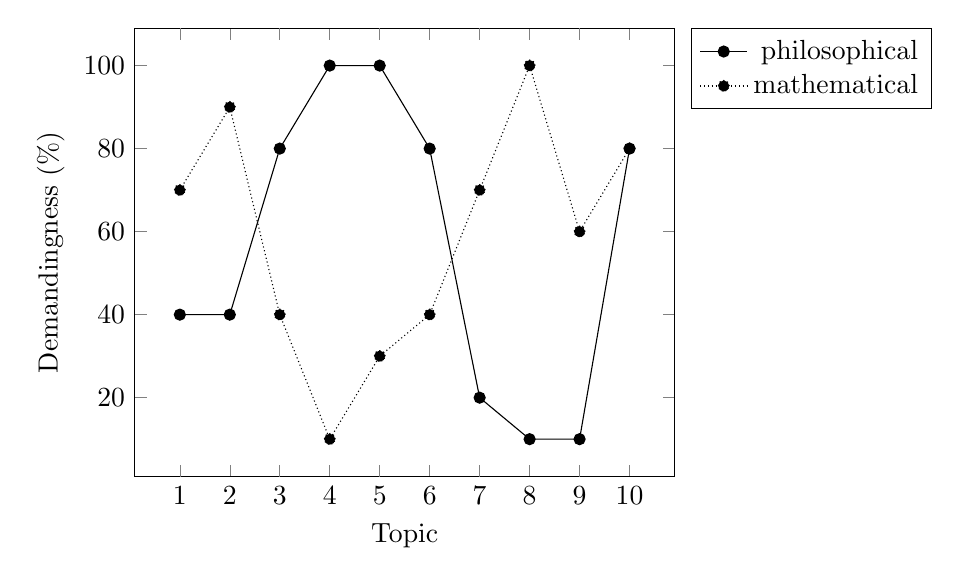
\begin{tikzpicture}
\begin{axis}[
	xlabel={Topic},
	ylabel={Demandingness (\%)},
	extra x ticks={1,3,5,7,9},
	legend style={
		cells={anchor=east},
		legend pos=outer north east,
	},
	cycle list={
		{black,mark=*},
		{densely dotted,mark=*}
	},
]
\addplot coordinates {
	(1,40) (2,40) (3,80) (4,100) (5,100) (6,80) (7,20) (8,10) (9, 10) (10, 80)
};

\addplot coordinates {
	(1,70) (2,90) (3,40) (4,10) (5,30) (6,40) (7,70) (8,100) (9,60) (10, 80)
};


\legend{philosophical, mathematical}
\end{axis}
\end{tikzpicture}
 
\end{center}


 \begin{itemize}
     \item On the \textbf{philosophical} side, a demandingness level of 100\% means that some of the ideas we'll be discussing are rather subtle; you won't need philosophical training to understand them, but you'll have to think about them very carefully.

\item On the \textbf{mathematical} side, a demandingness level of 100\% means that the lecture is designed for someone who is familiar with college-level mathematics or is otherwise experienced in mathematical proof.

 \end{itemize}

\vskip.15in
\noindent\textbf{Course Materials:}

The main course materials will be provided via MITx and can be accessed through Canvas. The materials include both videos and text. The most important part of the class is the written text. That's what you'll have to focus on if you want to understand the material. You don?t need to watch the videos if you don't want to.  

The MITx materials include videos of three different kinds:

\begin{itemize}
    \item  \emph{Lightboard videos:} I use these videos to go over the key concepts of the relevant lecture.  Although they overlap with the written text, I sometimes go about things in a slightly different way, in an effort to give you an alternate perspective.

\item \emph{Lectures from pre-pandemic times:} These videos often cover similar material to what you'll find in the text, but the material is sometimes presented a bit differently because I gave the lectures several years before I finalized the text.

\item \emph{Extras:} I posted these videos  in the hope that you might find them interesting or fun. (Sometimes they are interviews with experts in the field; sometimes they are introductions to a topic; sometimes they are animations made to help explain a point.)
\end{itemize}


In addition to the problem sets, which will be posted on Canvas, you'll find exercises scattered throughout the MITx lectures. \textbf{Your answers to these exercises will not count towards your final grade.} You shouldn't stress about the exercises, but you should give them a go: they'll deepen your understanding of the material and they are good preparation for problem sets. Some of exercises are quite hard. But, as I said, don't stress out about them. I felt free to make them hard because we knew they wouldn't be graded.

\vskip.15in
\noindent\textbf{Textbook:} %\footnotemark
There is no required textbook, as all course materials will be available on MITx. The MITx materials are based on the book below, which you can buy if you prefer a non-electronic format or if you'd like to retain access to the course materials after the end of the semester:

\vspace{3mm}
\begin{center}
  \includegraphics[width=3.5cm]{cover.png}\\
Rayo, A. \emph{On the Brink of Paradox}, MIT Press, 2019.\\
\end{center}





\vskip.15in
\noindent\textbf{Piazza Wiki:}
The class has a Piazza Wiki, which is accessible through Canvas. Please use the wiki to ask questions about the class and interact with your fellow students. (No answers to problem set questions please!) Posting on Piazza is one of two ways of earning discussion credit---see below.



\vskip.15in
\noindent \textbf{Course Schedule:}
The class is divided into 10 modules, which will be released sequentially throughout the semester. Each module has an MITx lecture and a problem set, with the exception of modules 7 and 8, which have separate lectures but a joint problem set. (See Canvas site for release dates and due dates.)



\vspace*{.15in}
\noindent\textbf{Grading Policy:} 
There will be no final examination. Final grades will be calculated as follows:


\begin{center} \begin{minipage}{3.0in}
\begin{flushleft}
Problem Sets \dotfill 85\% \\
%Pop Quizzes and Surveys \dotfill 15\% \\
Discussion \dotfill 15\% \\
\end{flushleft}
\end{minipage}
\end{center}
\vspace*{1mm}




\vskip.15in
\noindent\textbf{Problem Sets:} Problem sets will be posted on Canvas, and answers must be submitted on Canvas.  
Your submission must be a PDF file. 

Type-written submissions are strongly preferred. Handwritten submissions are only acceptable if: $(i)$ your handwriting is easily legible (as judged by your TA), $(ii)$ you produce a clean version of the document (as opposed to the sheet of paper you used to work out the problems), and $(iii)$ your manuscript has been scanned to high enough standards (as judged by your TA). Note, in particular, that {a garden-variety phone photo won't do}. If you must use your phone for scanning, please make sure you use a scanning app, such as \emph{Adobe Scan}, and make any necessary adjustments to the image before it is uploaded. If you are unsure whether your handwriting or your scanning technology will be up to your TA's standards, make sure you get guidance from them well in advance of the problem set's due date.

Your lowest problem set grade will be dropped. If you miss any additional problem sets, however, \textbf{you will not be able to make up for them.} So make sure you don't waste your freebee: keep it in store for when you really need it, which will almost certainly happen towards the end of the semester when your other classes start picking up and problem sets get more difficult.  \textbf{Late assignments will not be accepted.} 

Even though the class has 10 modules, there will be only 9 problem sets. This is because modules 7 and 8 will have a joint problem set. (The joint problem set isn't worth double: it's worth the same as an ordinary problem set.)



\begin{quote}

    

\emph{Collaboration Policy:} It's okay to discuss problem sets with other students who are currently taking the class, but \textbf{you must complete the problem set on your own and provide a list of commentators} by using the ``comment'' box on Canvas when you submit your problem set. If you collaborate, \textbf{failure to submit a list of commentators constitutes plagiarism.}
To make it easy for people to find collaboration partners, I've registered the class on:
\begin{center}
\url{https://psetpartners.mit.edu}
\end{center}

\vspace{2mm}

\emph{Anonymous Grading:} In an effort to mitigate bias, your TA will endeavour to grade each problem set without knowing the identity of its author. In order for this to be achievable, though, we need your help:

\begin{itemize}
    \item Please \underline{do not} include your name on problem set submissions: {include your MIT ID instead}.
    
    \item Please \underline{do not} list your collaborators on  problem set submissions. As explained above, you should list any collaborators using the ``comment'' box on Canvas, as you submit your problem set.
\end{itemize}

\vspace{2mm}



\emph{Policy on Outside Sources:} Consulting published materials is okay. With the exception of course-materials, all sources must be credited, in accordance with MIT's Academic Integrity guidelines. (Problem sets from previous versions of the class do not count as ``course materials" for present purposes and may not be consulted. Any violation of this policy will be considered plagiarism and will be  pursued aggressively.)

\end{quote}

\vskip.15in
\noindent\textbf{Discussion Credits:}  
You can receive up to 2 discussion credits for each module. There is no way to make up for missed discussion credits, but your worst module will be dropped from your discussion grade for the class.


There are two ways of earning discussion credits:
\begin{itemize}
    \item \emph{Attend recitation sections:} although section attendance is optional,  you can earn up to one discussion credit for attending your assigned recitation section from beginning to end and one additional credit for making a meaningful contribution to the discussion. (It is up to your TA to determine what counts as meaningful, but asking a thoughtful question and offering a thoughtful answer to someone else's question are both good examples of meaningful contributions.) 
    
    \item \emph{Be active on Piazza:} you can earn discussion credits for posting meaningful contributions to the online discussion forum, with each independent contribution worth one credit. (It is up to your TA to determine what counts as meaningful and what counts as independent; asking a thoughtful question, offering a thoughtful answer to someone else's question, and making an interesting comment are all good examples of meaningful posts.) A Piazza post is only eligible for discussion credit if it is posted to the entire class.
    
    
\end{itemize}
Keep in mind that you can earn no more than two discussion credits per module. A recitation section contribution can only count towards a given module's allotment if it takes place after the course materials for that module have been released and before the module's problem set is due. A Piazza contribution can only count towards a given module's allotment if it is on a topic directly connected to the relevant module and if it is posted at least 24 hours before the module's problem set is due. (When a single contribution might correspond to more than one section, you can choose to use your contribution towards the allotment of any of the relevant modules.)

It is your responsibility to inform your TA how you have satisfied each module's discussion credits. \textbf{You'll need to input the information on canvas}, by the due date of the relevant problem set. (Modules 7 and 8 have separate discussion credit allotments, even though they have a joint problem set.) Pleas keep in mind that misrepresenting your contributions constitutes an infringement of our academic integrity guidelines and can lead to disciplinary action.




\vskip.15in 
\noindent\textbf{Grading Scheme:}

\begin{center}\begin{minipage}{3.5in}\begin{multicols}{2}
\begin{flushleft}
\noindent
100\% \dotfill  A+\\
      94--99\% \dotfill A\mbox{\hspace{3mm}}\\
 90--93\% \dotfill A$-$\\
 89\% \dotfill B+\\
 84--88\% \dotfill B\mbox{\hspace{3mm}}\\
 80--83\% \dotfill B$-$\\
  79\% \dotfill C+\\
   74--78\% \dotfill C\mbox{\hspace{3mm}}\\
 70--73\% \dotfill C$-$\\
 60--69\% \dotfill D\mbox{\hspace{3mm}}\\
 0--60\% \dotfill F\mbox{\hspace{3mm}}
\end{flushleft}
\end{multicols}
\end{minipage}\end{center}

   






\vskip.15in
\noindent\textbf{Exceptions to class policy:} If there are exceptional circumstances that prevent you from submitting a problem set on time or earning discussion credits  (e.g.~a medical emergency), your first step should be to contact MIT's Student Support Services ($S^3$). If the $S^3$ Dean believes that your situation warrants an exception to standard class policies, please ask them to contact me requesting the exception. \textbf{I will not consider exceptions unless the request comes from $\bm S^3$}. (I strongly recommend that you contact $S^3$ \emph{before} your assignment is due.)


\vskip.15in
\noindent\textbf{Grade Adjustments:} If you feel like you got the wrong grade on an assignment and are not able to sort things out with your TA, you're welcome to send me your assignment for regrading. Please keep in mind, however, that this can cause your grade to go down rather than up. \emph{I am not as tenderhearted as some of my TAs.}

\vskip.15in
\noindent\textbf{Zoom Policy:} Office hours and recitation sections will be conducted by Zoom, which will be accessible through Canvas. Zoom sessions will not be recorded, so as to encourage participation. We much prefer it when students keep their video cameras on and are clearly visible on screen, so as to encourage a lively and friendly discussion. But students who would rather keep their camera off will not be penalized or singled out.
 

\vskip.15in
\noindent\textbf{Different Time Zones:} I am mindful of the fact that students may be working from different time zones during the pandemic and will do my best to ensure that office hours and recitation section times accommodate as many people as possible. If you are working from a different time zone and feel like you need some sort of accommodation, {please let me know during the first week of class} by taking the welcome survey, which is available through Canvas.

\vskip.15in
\noindent\textbf{Disability:}
Students with disabilities are welcome in this class. If you require an exception to class policies because of a disability, please contact Student Disability Services and ask them to send me a request on your behalf. 













\vskip.15in
\noindent\textbf{Academic Integrity:}  
 Any suspicion of plagiarism or academic dishonesty will be aggressively pursued. Please consult MIT's Guidelines on Academic Integrity: \url{https://integrity.mit.edu/}.










%%%%%% END 
\end{document} 